%% Dexter Barrows, 2016
%% dbarrows.github.io

\section{Spatial SIR}

	Spatial epidemic models provide a way to capture not just the temporal trend in an epidemic, but to also integrate spatial data and infer how the infection is spreading in both space and time. One such model we can use is a dynamic spatiotemporal SIR model.

	We wish to construct a model build upon the stochastic SIR compartment model described previously but one that consists of several connected spatial locations, each with its own set of compartments. Consider a set of locations numbered $i = 1, ..., N$, where $N$ is the number of locations. Further, let $N_i$ be the number of neighbours location $i$ has. The model is then

	\begin{equation}
		\begin{aligned}
			\frac{dS_i}{dt} & = - \left( 1 - \phi \frac{N_i}{N_i + 1} \right) \beta_i S_i I_i - \left( \frac{\phi}{N_i + 1} \right) S_i \sum_{j = 0}^{N_i} \beta_j I_j \\
			\frac{dI_i}{dt} & = \left( 1 - \phi \frac{N_i}{N_i + 1} \right) \beta_i S_i I_i + \left( \frac{\phi}{N_i + 1} \right) S_i \sum_{j = 0}^{N_i} \beta_j I_j - \gamma I \\
			\frac{dR_i}{dt} & = \gamma I,
		\end{aligned}
	\end{equation}
    
	Neighbours for a particular location are numbered $j = 1, ..., N_i$. We have a new parameter, $\phi \in [0,1]$, which is the degree of connectivity. If we let $\phi = 0$ we have total spatial isolation, and the dynamics reduce to the basic SIR model. If we let $\phi = 1$ then each of the neighbouring locations will have weight equivalent to the parent location.

	As before we let $\beta$ embark on a geometric random walk defined as

	\begin{equation}
		\beta_{i, t+1} = \exp \left( \log(\beta_{i, t}) + \eta (\log(\bar{\beta}) - \log(\beta_{i, t})) + \epsilon_{t} \right).
	\end{equation}
	
	Note that as $\beta$ is a state variable, each location has its own stochastic process driving the evolution of its $\beta$ state.

	If we imagine a circular topology in which each of $10$ locations is connected to exactly two neighbours (i.e. location $1$ is connected to locations $N$ and $2$, location $2$ is connected to locations $1$ and $3$, etc.), and we start each location with completely susceptible populations except for a handful of infected individuals in one of the locations, we obtain a plot of the outbreak progression in Figure [\ref{dataplot}].

	\begin{figure}[H]
        \centering
        \captionsetup{width=.8\linewidth}
        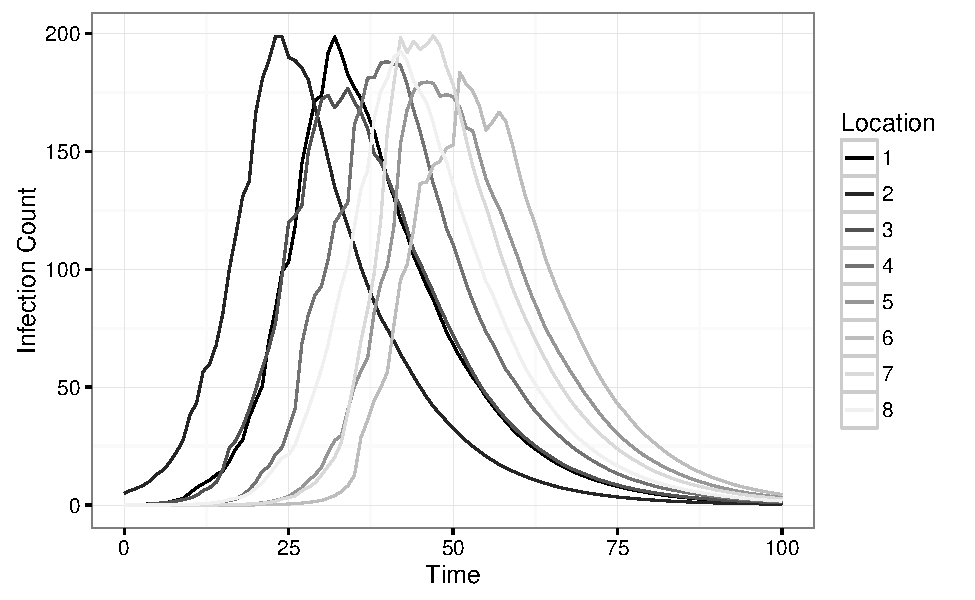
\includegraphics[width=0.8\textwidth]{./images/dataplot.pdf}
        \caption{Evolution of a spatial epidemic in a ring topology. The outbreak was started with 5 cases in Location 2. Parameters were $R_0 = 3.0$, $\gamma = 0.1$, $\eta = 0.5$, $\sigma_{err} = 0.5$, and $\phi = 0.5$.}
        \label{dataplot}
    \end{figure}

    If we add noise to the data from Figure [\ref{dataplot}], we obtain Figure [\ref{dataplot2}], below.

    \begin{figure}[H]
        \centering
        \captionsetup{width=.8\linewidth}
        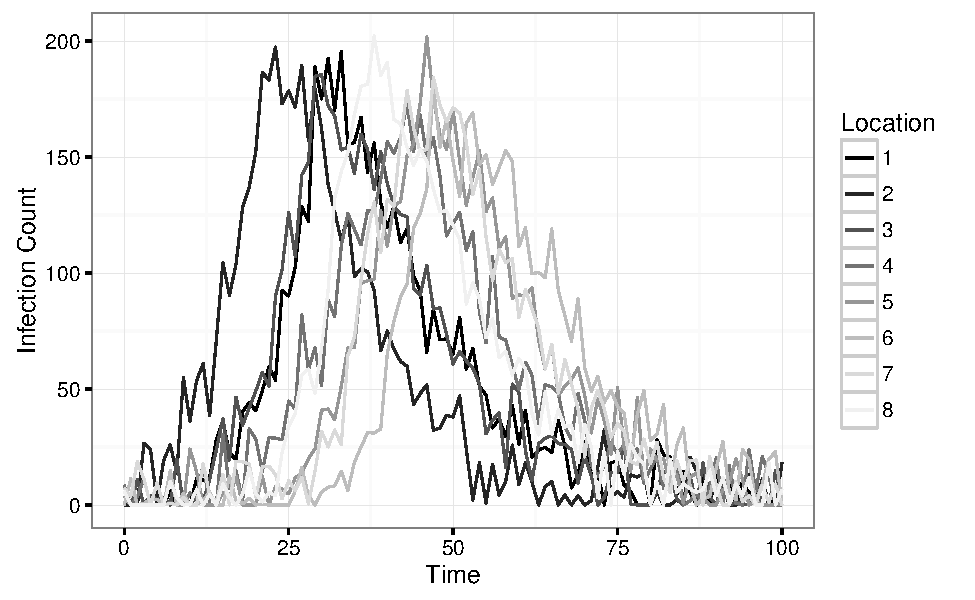
\includegraphics[width=0.8\textwidth]{./images/dataplot2.pdf}
        \caption{Evolution of a spatial epidemic as in Figure [\ref{dataplot}], with added observation noise drawn from $\mathcal{N}(0,10)$.}
        \label{dataplot2}
    \end{figure}


\section{Dewdrop Regression}

	Dewdrop regression (references) aims to overcome the primary disadvantage suffered by methods such as the S-map or its cousin Simplex Projection: the requirement of long time series from which to build a library. Suggested by Sugihara's group in 2008, Dewdrop Regression works by stitching together shorter, related, time series, in order to give the S-map or similar methods  enough data to operate on. The underlying idea is that as long as the underlying dynamics of the time series display similar behaviour (such as potentially collapsing to the same attractor), they can be treated as part of the same overarching system.

	It is not enough to simply concatenate the shorter time series together -- several procedures must be carried out and a few caveats observed. First, as the individual time series can be or drastically differing scales and breadths, they all must be rescaled to unit mean and variance. Then the library is constructed as before with an embedding dimension $E$, but any library vectors that span any of the seams joining the time series are discarded. Further, and predictions stemming from a library vector must stay within the time series from which they originated. In this way we are allowing the ``shadow'' of of the underlying dynamics of the separate time series to infer the forecasts for segments of other time series. Once the library has been constructed, S-mapping can be carried out as previously specified.

	This procedure is especially well-suited to a the spatial model we are using. While the dynamics are stochastic, they still display very similar means and variances. This means the rescaling process in Dewdrop Regression is not necessary and can be skipped. Further, the overall variation between the epidemic curves in each location is on the smaller side, meaning the S-map will have a high-quality library from which to build forecasts.


\section{Spatial Model Forecasting}

	In order to compare the forecasting efficacy of Dewdrop Regression with S-mapping against IF2 and HMCMC, we generated 20 independent spatial data sets up to time $T = 50$ weeks in each of $L = 10$ locations and forecasted $10$ weeks into the future. Forecasts were compared to that of the true model evolution, and the average $SSE$ for each week ahead in the forecast were computed. The number of bootstrapping trajectories used by IF2 and HMCMC was reduced from 200 to 50 to curtail running times.

	The results are shown in Figure [\ref{sseplot}]. 

	\begin{figure}[H]
        \centering
        \captionsetup{width=.8\linewidth}
        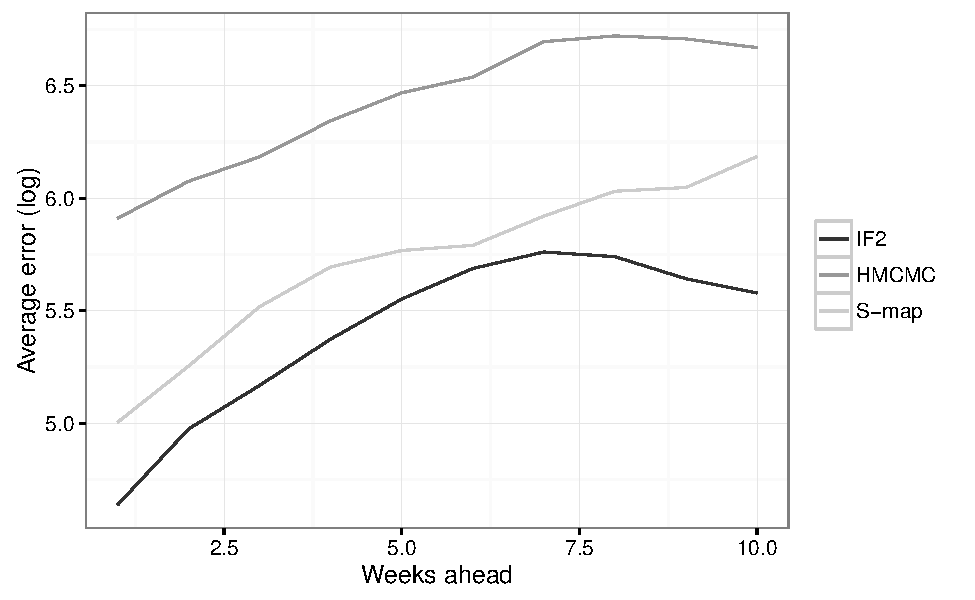
\includegraphics[width=0.8\textwidth]{./images/sseplot.pdf}
        \caption{Average SSE (log scale) across each location and all trials as a function  of the number of weeks ahead in the forecast.}
        \label{sseplot}
    \end{figure}

    The results show a clear delineation in forecast fidelity between methods. IF2 maintains an advantage regardless of how long the forecast produced. Interestingly, Dewdrop Regression with S-mapping performs almost as well as IF2, and outperforms HMCMC. HMCMC lags behind both methods by a healthy margin.

    If we examine the runtimes for each forecast framework, we obtain the data in Figure [\ref{timeplot}].

    \begin{figure}[H]
        \centering
        \captionsetup{width=.8\linewidth}
        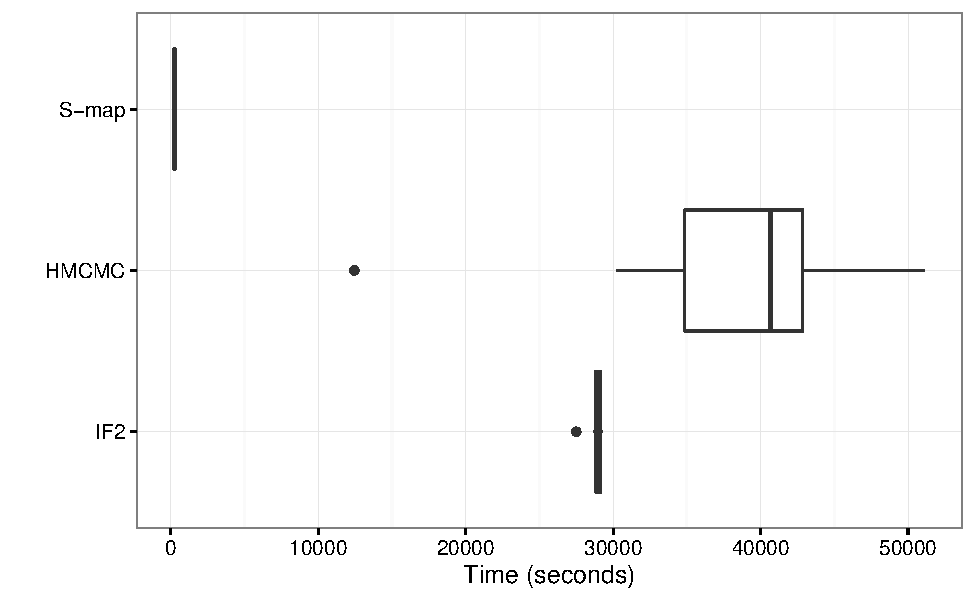
\includegraphics[width=0.8\textwidth]{./images/timeplot.pdf}
        \caption{Runtimes for producing spatial SIR forecasts. The box shows the middle 50th quantile, the bold line is the median, and the dots are outliers.}
        \label{timeplot}
    \end{figure}

    As before, the S-map with Dewdrop Regression runs faster than the other two methods with a huge margin. It is again hard to see exactly how large the margin is from the figure due to the scale, but we can examine the average values: the average running time for S-mapping with Dewdrop Regression was about $249$ seconds, whereas the average times for IF2 and HMCMC were about $2.90 \times 10^4$ and $3.88 \times 10^4$, respectively. This is a speed-up of just over 116x over IF2 and 156x over HMCMC.

    Considering how well S-mapping performed with regards to forecast error, it shows a significant advantage over HMCMC in particular -- it outperforms it in both forecast error and running times.
